\documentclass[a4paper, 12pt, oneside]{book}

\pagestyle{myheadings}

\usepackage[T1]{fontenc}
\usepackage{ae}
\usepackage[utf8]{inputenc}
\usepackage[brazilian]{babel}
\usepackage{graphicx}
\usepackage{hyperref}

\linespread{1.5} 
\setlength{\hoffset}{-1in}
\setlength{\oddsidemargin}{3.0cm} 
\setlength{\textwidth}{160mm} 
\setlength{\parindent}{1.25cm} 
\setlength{\voffset}{-1in}
\addtolength{\voffset}{2.0cm}
\setlength{\topmargin}{0.0cm}
\setlength{\headheight}{5mm}
\setlength{\headsep}{5mm}
\setlength{\textheight}{247mm} 

%%%%%% COMPLETAR DADOS AQUI %%%%%%%%%%%
\def\titulo{Simulando Algoritmos Quânticos em um
Computador Clássico}
\def\tituloEN{Simulating Quantum Algorithms in a clássical
Computer}
\def\nome{Igor Valente Blackman}
\def\ano{2017}

\begin{document}

%%%%%%%%%%%%%%%%%%%%%%%%%%%%%%%%%%%%%%%%%%%%%%%
%     CAPA

\begin{titlepage}
 \noindent 
 \rule{\textwidth}{1ex} \\ [1ex]
 \begin{center}
  \begin{minipage}{0.15\textwidth}
   
\includegraphics[width=1\textwidth]{./logoUFF.png} 
  \end{minipage}
  \begin{minipage}{0.65\textwidth}
   \centering
   {\large \textsc{Universidade Federal Fluminense} } \\ [1.5ex]
   {\large \textsc{Instituto de Computação} } 
  \end{minipage}
  \begin{minipage}{0.15\textwidth}
   
\includegraphics[width=1\textwidth]{./logoIC.png}
  \end{minipage}
    
  \vfill
  {\Huge \textbf{\titulo}} \vfill
  {\huge \nome} \\ [25ex]
  {\large NITERÓI - RJ} \\ [1.5ex]
  {\large \ano}
 \end{center}\vspace{1ex}
 \rule{\textwidth}{1ex}
\end{titlepage}

%%%%%%%%%%%%%%%%%%%%%%%%%%%%%%%%%%%%%%%%%%%%%%%
%    CONTRA - CAPA

\begin{titlepage}
  \begin{center}
    \Large{\textsc{Universidade Federal Fluminense} \\
           \textsc{Instituto de Computação} \\ 
           \textsc{Departamento de Ciência da Computação} 
          }
    \par\vfill
    \LARGE{\nome}
    \par\vfill
    \LARGE{\titulo}
    \par\vfill
    \Large{NITERÓI - RJ \\
    \ano}
  \end{center}
\end{titlepage}

\pagenumbering{roman}
\setcounter{page}{2}

%%%%%%%%%%%%%%%%%%%%%%%%%%%%%%%%%%%%%%%%%%%%%%%
%    FOLHA DE ROSTO

\begin{center}

\MakeUppercase{\nome}

\vfill

\MakeUppercase{\titulo}

\vspace{3.0cm}

\begin{flushright}
\begin{minipage}{0.50\textwidth}

Trabalho submetido ao Curso de Bacharelado em Ciência da Computação da Universidade Federal Fluminense como requisito parcial para a obtenção do título de Bacharel em Ciência da Computação.

\end{minipage}
\end{flushright}

\vspace{3.0cm}

Orientadora: Profa. Dra. Karina Mochetti de Magalhães

\vfill

Niterói - RJ \\
\ano

\end{center}

\newpage

%%%%%%%%%%%%%%%%%%%%%%%%%%%%%%%%%%%%%%%%%%%%%%%%%%%%%    FICHA CATALOGRÁFICA

\newpage

%%%%%%%%%%%%%%%%%%%%%%%%%%%%%%%%%%%%%%%%%%%%%%%%%%%%%    FOLHA DE APROVAÇÃO

\newpage

%%%%%%%%%%%%%%%%%%%%%%%%%%%%%%%%%%%%%%%%%%%%%%%%%%%%%    DEDicatória

\begin{flushright}
\begin{minipage}{0.5\textwidth}

\vspace{15.0cm}

\emph{
Dedicatória
}

\end{minipage}
\end{flushright}

%%%%%%%%%%%%%%%%%%%%%%%%%%%%%%%%%%%%%%%%%%%%%%%%%%%%%    AGRADECIMENTOS

\chapter*{Agradecimentos}
\addcontentsline{toc}{chapter}{Agradecimentos}

\thispagestyle{myheadings}

\noindent

Agradecimento 1.

\ \\ 

Agradecimento 2.

\ \\ 

...

\ \\ 

Agradecimento N.

%%%%%%%%%%%%%%%%%%%%%%%%%%%%%%%%%%%%%%%%%%%%%%%%%%%%%    RESUMO

\chapter*{Resumo}
\addcontentsline{toc}{chapter}{Resumo}

\thispagestyle{myheadings}

A construção de um computador quântico terá impactos profundos em várias áreas, tais como Física, Matémática e, especialmente, a Ciência da Computação. As dificuldades práticas para se construir um computador quântico são muitas, logo não é possível prever quando ou mesmo se um computador quântico será construído. Apesar disso, a teoria na área da computação quântica vem evoluindo fortemente e para auxiliar na análise desses algoritmos pode ser essencial a criação de um simulador quântico de fácil acesso. Esse simulador utilizaria um computador clássico para realizar os trabalhos de um computador quântico, simulando o entrelaçamento e a sobreposição em bits clássicos e realizando uma estimativa de tempo gasto num computador quântico. O objetivo desse trabalho é realizar a implementação de um simulador para algoritmos quânticos.

\ \\

Palavras-chave: PALAVRA1, PALAVRA2, PALAVRA3. 

%%%%%%%%%%%%%%%%%%%%%%%%%%%%%%%%%%%%%%%%%%%%%%%%%%%%%    ABSTRACT

\chapter*{Abstract}
\addcontentsline{toc}{chapter}{Abstract}

\thispagestyle{myheadings}

The construction of a quantum computer will have deep impacts in several áreas, such as Physics, Mathematics, and especially Computer Science. There are several practical difficulties in building a quantum computer, so it is not possible to predict when or even if a quantum computer will be built. Nevertheless, the theory in the Quantum Computing field is evolving strongly and to assist in the analysis of these algorithms can be essential to creaté a quantum simulator. This simulator would be implemented in a classic computer, performing the work of a quantum computer, simulating the superposition and entanglement in clássical bits with an estimaté of efficiency. Therefore, the aim of this work is implement a simulator for quantum algorithms.

\ \\

Keywords: WORD1, WORD2, WORD3.

%%%%%%%%%%%%%%%%%%%%%%%%%%%%%%%%%%%%%%%%%%%%%%%%%%%%%    SUMן�½RIO

\tableofcontents

\thispagestyle{myheadings}

%%%%%%%%%%%%%%%%%%%%%%%%%%%%%%%%%%%%%%%%%%%%%%%%%%%%%    LISTA DE FIGURAS

\listoffigures
\addcontentsline{toc}{chapter}{Lista de Figuras}

\thispagestyle{myheadings}

%%%%%%%%%%%%%%%%%%%%%%%%%%%%%%%%%%%%%%%%%%%%%%%%%%%%%    LISTA DE TABELAS

\listoftables
\addcontentsline{toc}{chapter}{Lista de Tabelas}

\thispagestyle{myheadings}

%%%%%%%%%%%%%%%%%%%%%%%%%%%%%%%%%%%%%%%%%%%%%%%%%%%%%    TEXTO

\pagebreak
\pagenumbering{arabic}

\chapter{Introdução}
\thispagestyle{empty}

A computação quântica aproveita a possibilidade de que as particulas subatômicas podem ter mais de um estado a qualquer momento~\cite{wiredQC}. Em um computador normal, que chamaremos de clássico, um bit é um simples pedaço de informação que possui apenas dois estados, 0 ou 1. Para representar tal informação um computador deve conter algum tipo de sistema físico com dois estados distintos para associar aos valores como, por exemplo um switch que pode estar fechado (1) ou aberto (0)~\cite{mermin}.

Computadores quânticos utilizam bits quânticos ou "qubits", sistemas quânticos que também possuem dois estados, entretanto, diferente do bit clássico qubits podem armazenar muito mais informação já que eles podem existir em qualquer sobreposição desses valores, 0 ou 1, ou ambos ao mesmo tempo~\cite{wiredQC}. 

No mundo da mecânica quântica os eventos são governados por probabilidades. Um átomo radioativo, por exemplo, pode enfraquecer emitindo um eletron, ou não. É possível preparar um experimento de tal forma que exista uma chance exata de 50\% de que um dos átomos de um pedaço de matérial radioativo caia em um determinado tempo~\cite{gribbin}.

Pode-se tomar como exemplo o experimento teórico do "Gato de Schrödinger". São colocados um gato, um frasco de veneno e uma fonte de radiação em uma caixa selada. Se um monitor interno (ex. Contador Geiger) detecta radiação, o frasco é quebrado soltando o veneno, matando o gato. No mundo clássico existe uma chance de 50\% de o gato estar morto, e sem olhar dentro da caixa podemos dizer que o gato está vivo ou morto. Segundo a teoria, nenhuma das duas possibilidades tem qualquer realidade a menos que seja observada~\cite{gribbin}. Isso se equivale para o qubit, ele pode ser 0 ou 1 ao mesmo tempo mas quando ele é observado ele deixa de ser um bit quântico e passa a ser um bit clássico, ou seja, só pode ser 0 ou 1.

Outra visão quanto a um qubit pode-se pensar em uma esfera imaginaria onde um bit clássico pode estar apenas em um dos polos da esfera e o qubit, bit quântico, pode estar em qualquer ponto da esfera. Assim qubits podem armazenar uma quantidade muito maior de informação que um bit clássico.

\section{Motivação e Objetivo}

A computação quântica é uma área de pesquisa muito relevante, pois utiliza elementos de três áreas importantes: como a Física, Matémática e Engenharia. Apesar de ainda não ser possível prever quando ou mesmo se um computador quântico será construído, caso isto ocorra serão gerados grandes impactos em todas essas áreas. Em um computador quântico, os sistemas não devem ter interações físicas que não sejam sob o controle total e completo do programa. Diferente de como ocorre em um computador comum, ou os chamados computadores clássicos, interações físicas não controladas introduziriam interrupções potencialmente catastróficas na operação de um computador quântico, o que resulta numa dificuldade na construção do mesmo. 

Entretanto, os benefícios que podem ser gerados com a construção de um computador quântico vão muito além do que os pesquisadores podem imaginar. Para os cientistas da computação, o mais impressionante na computação quântica e a eficiência alcançada por seus algoritmos, algo não possível na teoria clássica da complexidade computacional. O tempo de execução de algumas tarefas em um computador quântico cresce de forma muito mais lenta com o tamanho da entrada do que em um computador clássico. 

Neste trabalho apresentamos a implementação de um simulador de circuitos quânticos que utiliza um computador clássico para executar os algoritmos em um computador quântico. Assim, características quânticas como o entrelaçamento e a sobreposição serão realizadas em bits clássicos o que resultará num gasto de tempo maior. Por isso, o simulador também gera uma estimativa de tempo gasto a partir das portas quânticas, emulando o que seria obtido por um computador quântico caso ele seja construído. As portas e o tempo gasto em cada uma e dado pelo usuário. O simulador é uma ferramenta online e dispõe de arraste das portas quânticas para formação dos circuitos com o intuito de facilitar a interação com o usuário.

\section{Revisão Bibliográfica}

\subsection{Quantum - Davy Wybiral}

Existe um simulador online desenvolvido por Davy Wybiral de Austin Texas, Quantum ou como está no projeto dele do Git Quantum Circuit Simulator~\cite{davyw}. O projeto foi disponibilizado no Git em Janeiro de 2017~\cite{gitdavyw}. Davy Wybiral utiliza o Canvas para gerar toda a parte gráfica dos circuitos e menus, e javascript para toda a parte de cálculo. O simulador não possui nenhum tipo de documentação e tem uma interface bem simples com um menu superior onde existem algumas opções e uma área com as portas quânticas que podem ser adicionadas nos circuitos e ter a quantidade dos mesmos alterada.

\begin{figure}[hbtp]
\centering
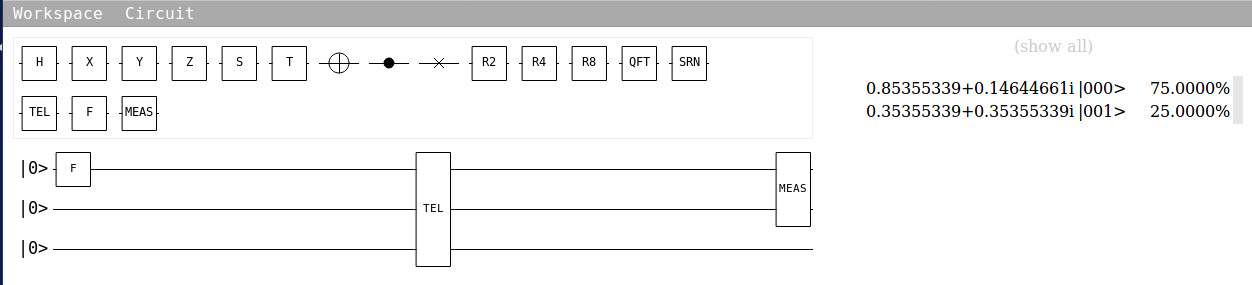
\includegraphics[scale=0.36]{davyw.jpg}
\caption{Simulador quântico de Davy Wybiral}
\end{figure}

A montagem do circuito funciona com a seleção de uma das portas e após isso basta clicar nos circuitos para adicionar a porta selecionada. Pode-se deletar uma porta clicando com o botão direito. Nos casos de portas de 2-bits é necessário que haja uma ação de clique e arraste onde o clique seleciona a posição do bit de controle e ao largar fica a porta. Existe também a possibilidade de arrastar com uma porta de 1-bit selecionada o que adiciona a mesma em diversos circuitos.

Para efetuar o cálculo do circuito basta pressionar a tecla Enter ou selecionar no menu a opção Evaluaté. O resultado é mostrado ao lado direito com todas as possibilidades possíveis e suas respectivas probabilidades.

\subsection{Quirk - Craig Gidney}

O projeto teve seu início em Março de 2014 mas não teve commits após o mes de criação. Em Novembro do mesmo ano, 2014, voltou a ter commits e entre Março de 2016 e Novembro de 2016 foi quando se teve a maior concentração de commits, 647 dos 1006 totais. O projeto ainda vem sendo atualizado sendo o commit mais recente do dia 29 de Abril de 2017~\cite{gitquirk}. Craig Gidney, desenvolvedor do Quirk, explica que decidiu criar o simulador porque ficou interessado em computação quântica e pelo fato de ter lido "Media for Thinking the Unthinkable" de Bret Victor onde ele menciona benefícios do feedback imediato em relação ao entendimento e produtividade. Craig diz não ter achado nenhum simulador de circuitos quânticos que passasse essa experiência de "manipulação direta"~\cite{quirk}. Foi desenvolvido utilizando Webgl.

\begin{figure}[hbtp]
\centering
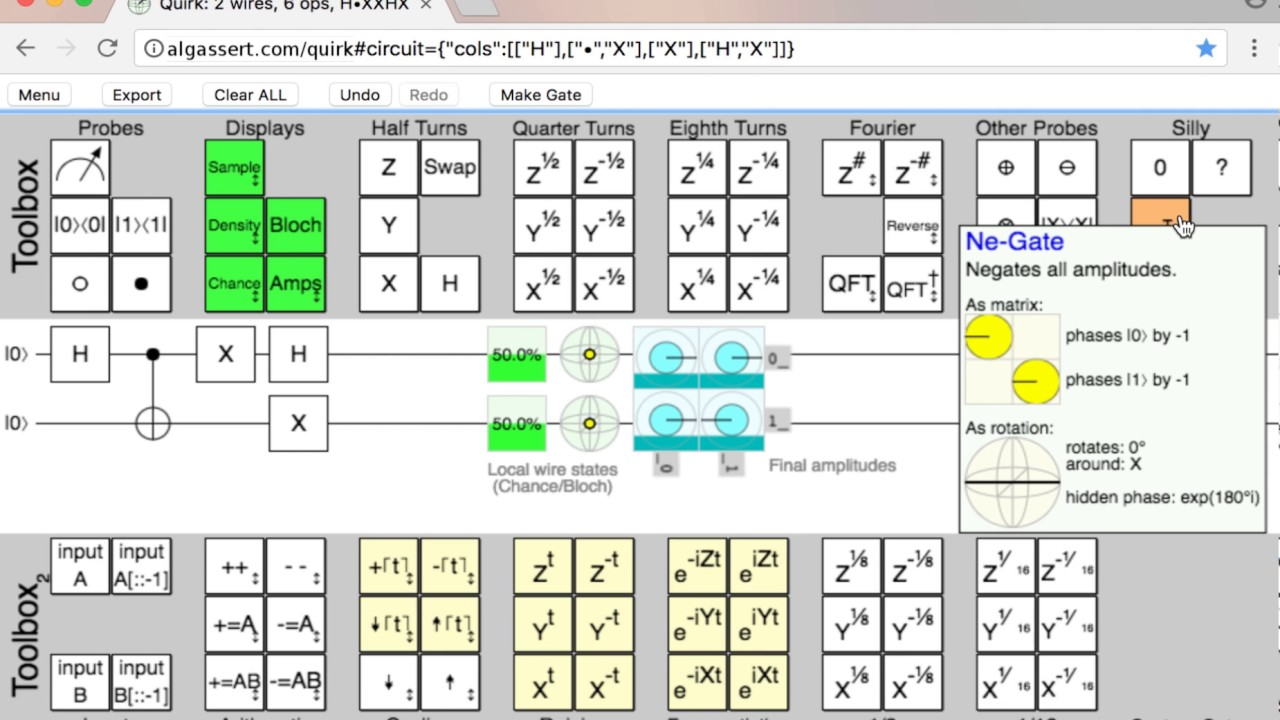
\includegraphics[scale=0.36]{quirk.jpg}
\caption{Simulador quântico Quirk de Craig Gidney}
\end{figure}

Craig faz comparações com alguns simuladores como por exemplo o já mencionado de Davy Wybiral e o IBM Quantum Experience. Ele também menciona alguns outros como Quantum Computing Playground e Microsoft's LIQ Ui|>.

O simulador Quirk é composto por um menu que possui opções de carregar alguns exemplos de circuitos já prontos, exportar o circuito montado, desfazer ou refazer alguma alteração e inclusive criar porta. Ele possui uma área com as opções de portas a serem utilizadas no circuito, formas de mostrar o resultado e mais diversas opções. Algumas vantagens desse simulador são: as portas são colocadas da forma "arrastar e soltar", o resultado é mostrado a todo momento não havendo a necessidade de se apertar um botão para isso, e é possível adicionar mais bits ao circuito dinâmicamente com o arrastar de uma das portas para além da linha do último bit.

\section{Organização do Texto}

Este trabalho está divido da seguinte forma: a Seção 2 é apresentada a motivação; na Seção 3 é realizada uma revisão bibliográfica, expondo a teoria e os frameworks existentes atualmente; a Seção 4 apresenta a solução implementada; a Seção 5 traz os resultados obtidos com o trabalho; e por final na Seção 6 são apresentadas as conclusões e trabalhos futuros.

\chapter{Escolha das ferramentas}
\thispagestyle{empty} 

\section{Linguagem}

Python foi a escolha por ser um linguagem com a qual tinhamos interesse de aprender e que é vastamente utilizada em diversas aplicações e empresas como: YouTube, Google, Industrial Light e Magic, etc...~\cite{pythonquotes} O que adiciona mais valor ao seu aprendizdo além de possuir todos os requisitos necessários para o desenvolvimento do projeto, frameworks de desenvolvimento web e bibliotecas de circuitos quânticos.

\section{Biblioteca}

Tendo em vista que escolhemos python como linguagem achamos algumas bibliotecas para a mesma:
\subsection{PyQu}
PyQu é um módulo de extensão para Python 3 com o objetivo principal de providenciar um completo conjunto de tipos de dados e funções para simular computação quântica com uma sintaxe pura. Entretanto o último commit feito foi a 7 anos o que nos fez entender que o projeto foi descontinuado, fazendo com que discartassemos essa opção~\cite{pyqu}.

\subsection{Qitensor}
Qitensor outro módulo que essencialmente é um pacote para Numpy~\cite{numpy} que utiliza semânticas mais úteis para mecânica quântica de dimensões finitas de muitas partículas. Mas essa biblioteca também não recebia atualizações a mais de ano~\cite{qitensor}.
\subsection{Qubiter}
Qubiter tinha como intuíto ajudar no designer e simulação de circuitos quânticos em computadores clássicos. É um projeto gêmeo do Quantum Fog e eles esperam que um dia o Quantum Fog chame o Qubiter para realizar algumas tarefas, como compilação e simulação quântica~\cite{qubiter}.	

\subsection{QuTiP}
QuTiP teve sua primeira versão em Julho de 2011~\cite{qutipchangelog}. É um software open-source para simular as dinâmicas de um sistema quântico aberto que utiliza os pacotes numéricos Numpy, Scipy e Cython. Teve sua primeira versão em Julho de 2011. Possui também um output gráfico provido pela Matplotlib. QuTiP tem como objetivo providenciar simulações numéricas eficientes e amigáveis para o usuário de um variado numero de Hamiltonianas comumente achadas em uma vasta quantidade de aplicações físicas. Está disponível sem custos para Linux, Mac OSX e Windows, sendo esta última com algumas restrições~\cite{qutip.org}. 

No site eles pedem para citar da seguinte forma.
J. R. Johansson, P. D. Nation, and F. Nori: "QuTiP: An open-source Python framework for the dynamics of open quantum systems.", Comp. Phys. Comm. 183, 1760–1772 (2012) [DOI: 10.1016/j.cpc.2012.02.021]. 

\section{Framework}

Sobre os Frameworks ficamos na dúvida entre 3 opções, Flask, Pyramid e Django.
\subsection{Flask}
Flask é o mais novo dentre os três, foi criado em meados de 2010. Teve o aprendizado dos frameworks que vieram antes dele e tem se destacado em pequenos projetos. Quanto a sua comunidade, é pequena se comparada à do Django mas é bem ativa em suas listas de email e no IRC~\cite{ryanbrown}. 

\subsection{Pyramid}
O Pyramid foi criado a partir do projeto Pylons~\cite{pylonsproject} e recebeu o nome de Pyramid no ano de 2010, mesmo tendo sua primeira realease em 2005. É um framework tão maduro quanto o Django e disponibiliza mais flexibilidade para desenvolvedores que possuem projetos onde o caso de uso não se encaixe muito bem nos padrões do mapeamento objeto-relacional~\cite{pyramid}. Pode-se dizer que Pyramid é o framework mais flexível dentre os três o que é um ponto positivo mas foi negativo para a escolha do framework, pois apresenta muitas opções para se começar um projeto. Além disso como pode-se ver mais a frente no trabalho possui a menos comunidade dentre os frameworks pesquisados.

\subsection{Django}
Django foi lançado em 2005. É um framework com foco em grandes aplicações, inclui dezenas de extras que podem ser usados para lidar com as tarefas comuns do desenvolvimento web, como por exemplo autenticação, administração de conteúdo, etc. Além de ajudar também com questões de segurança como SQL injection com seus querysets, evitar ataques Cross Site Scripting, proteção a Clickjacking, dentre outros~\cite{django}. De longe Django é o framework mais popular e a lista de sites que o utilizam é impressionante, mais de 5000~\cite{listadjangosites}. Para sites que possuem requisitos comuns, Django segue padrões bem sensatos tornando-o uma escolha bem popular entre media e grandes aplicações web.

\subsection{Comunidade}
Django possui uma quantidade enorme de perguntas no StackOverflow se comparado com os outros dois Frameworks, Django 144.000, Flask 16.600, Pyramid 1.900 (Maio 2017)~\cite{stackoverflowtags}. Mas já no Github Flask e Django têm números semelhantes e Pyramid 10 vezes menos, Flask possui um pouco mais de 27.200 estrelas, Django pouco mais de 25.900 e Pyramid 2.300~\cite{github}.

\subsection{Escolhido}
O Flask seria uma boa opção entretanto escolhemos o Django por: possuir a maior comunidade; diversas ferramentas já inclusas não tendo que "reinventar a roda"; ele foi criado para projetos escaláveis pensando em uma futura continuação do Projeto Final; força boas práticas no desenvolvimento além de ser uma ferramenta muito utilizada no mercado o que nos fez acreditar que traria mais benefícios com o aprendizado.

\chapter{Desenvolvimento}
\thispagestyle{empty} 

\section{Drag and Drop}

Como o simulador deveria ser amigável para o usuário decidimos em utilizar Drag \& Drop (D \& D) para a criação/edição do circuito. Resolvemos que o simulador deveria ter uma área com as portas quânticas disponíveis para montar o circuito quântico e a paritr dessa area o usuário poderia arrastar as portas para formar o circuito. Entretanto os D \& D convencionais apenas possibilitavam o arrastar de um elemento para um outro container, ou seja, o elemento deixava de existir no container original e era adicionado no final. O que queriamos era que o elemento inicial continuasse existindo onde estava e que uma cópia do mesmo fosse criada e adicionada ao container alvo, ou final, por isso decidimos criar um.

-----------

Tive varios problemas com a implementação do Drag and Drop, o que achei na internet apenas movia um elemento de um lugar para o outro mas nao era bem isso que eu queria.

No lugar inicial sempre tinha que ter a imagem e eu poderia arrasta-la para um dos pontos do circuito para assim montar o mesmo.

Entao vi que, ao iniciar o drag, nao deveria mover o objeto e sim criar uma copia dele e mover a copia.

Mas ao fazer isso acabei gerando novos problemas: 
\begin{itemize}
\item eu conseguir colocar diferentes imagens na mesma div, o que meio que gerava uma pilha, e a ideia nao era essa, em cada div do circuito deveria haver apenas 1 imagem. Entao tive que adicionar o tratamento do Drop para que a imagem já existente fosse deletada e ai sim adicionada a que foi arrastada até la.
\item As imagens se moviam de uma div do circuito para outra do circuito, o que resolvi fazendo com q a div apenas possuisse o evento de drop
\end{itemize}
	
Do matérial que achei na internet o JavaScript utilizado usava o ev.target o que gerava alguns problemas no tratamento do drop, pois esse target era o elemento sobre o qual o drop ocorreu, independente se o elemete possuia o evento de drop ou nao, o que me gerou confusao, mas acabei resolvendo o problema trocando target por currentTarget

\section{Iframe ou Div}

Objetivo inicial: Facilitar a visualização e utilização do simulador para montar os circuitos, com a existencia de scrolls latérais.

-Primeira solução foi englobar a div com uma div onde seriam aplicados as propriedades overflow e fixar a width e height. Mas com isso os novos circuitos nao aparecem, entao proximo passo seria modificar a altura da div quando um novo circuito e criado.

-foram criadas 2 funcoes para alterar a altura da div de acordo com a adicao ou exclusao de um circuito. Acabei utilizando a funcao outerHeight() do Jquery para pegar a altura total do circuito, quando estava usando apenas a funcao height() após acrescentar alguns circuitos o aumento nao era proprocional pois nao pegava os valores como padding, border, etc.

-foi criado tbm a funcao de ajustar width, para alterar a largura da div que contem os circuitos dependendo do numero de portas que os circuitos podem ter


\section{Ajax}

Escolhi fazer o cálculo do circuito por ajax para apenas alterar o resultado sem haver a necessidade de recarregar a pagina inteira. (1) Precisei fazer o tratamento do circuito para um objeto Json que seria passado para o ajax. (2) O sistema recebendo esse objeto utiliza a lib de python e calcula o circuito retornando o resultado. (3) Mostra o resultado na tela

(1)Tive varios problemas para entender como funcionava a parte de request do Django, entender o objeto QueryDict que e como o Django recebe o JSon enviado pelo Ajax. Tive que fazer tratamento para leitura, pois ele le de uma forma estranha.

https://docs.djangoproject.com/en/1.11/ref/request-response/

(2)Tive muita dificuldade para fazer a importação da lib Qutip no projeto, resolvendo as dependencias ta no OBS. Resolvi fazer o tratamento e criar uma funcao para realizar a transformação dependendo da porta (string) passada.

(3) O cálculo do tempo esta sendo feito pelo javascript pois já possuo todos os dados necessários na tela, nao existe a necessidade de enviar para o sistema. O sistema no passo anterior (2) processou os dados e retorna o resultado que e mostrado na tela.

OBS: Tive muito problema para arrumar as dependencias da lib Qutip
http://qutip.org/docs/3.1.0/installation.html

\section{Hospedagem - Heroku}

-criei um novo virtualenv para usar apenas as dependências necessárias
-após o projeto estar rodando localmente gerei o arquivo requirements.txt igual ao pio freeze daquele env.
-adicionei um arquivo runtime.txt para especificar a versão do python a ser utilizada, python-2.7.13 (heroku só aceita algumas versões, ele tem isso no site)
-criei o Procfile com apenas "web: gunicorn quantum-circuit-simulator.wsgi --log-file -" comando a ser executado qnd a aplicação começar a rodar
-logei e criei uma aplicação no heroku, "heroku creaté demo-quantum "
-especificquei o build pack, "heroku buildpacks:set heroku/python"
-addicionei e commitei as alterações feitas e realizei o deploy, "git push heroku master"
-Tirando os erros no processo, esses foram basicamente os passos
PS:
-Para instalar todas as dependências tive que fazer o deploy duas vezes alterando o requirements.txt porque não consegui achar uma forma de fazer a instalação do qutip por último e por isso acabava dando erro na instalação dele falando q faltavam dependência mas apenas prq na ordem de instalação elas não estavam sendo instaladas antes, primeiro deploy com a qutip comentado e segundo com ela, onde apenas ela foi instalada
-aprendi a escrever requirements hahaha (fiquei MT tempo sem conseguir fazer o deploy prq eu havia escrito requirements errado e não consegui reparar nisso


\chapter{Resultados}
\thispagestyle{empty} 

Texto...

\chapter{Conclusão e Trabalhos Futuros}
\thispagestyle{empty} 

Texto...
\cite{mermin}
\cite{qutip.org}
\cite{test2}
\cite{davyw}
\cite{quirk}
\cite{simulatorList}

%%%%%%%%%%%%%%%%%%%%%%%%%%%%%%%%%%%%%%%%%%%%%%%%%%%%%    REFERÊNCIAS BIBLIOGRÁFICAS
\bibliographystyle{plain}
\bibliography{monografia}



\end{document}


